\RequirePackage[hyphens]{url}
\documentclass[10pt, hyperref={unicode}]{beamer}
\PassOptionsToPackage{hyphens}{url}\usepackage{hyperref}
\usepackage{times}
\usepackage[slovak]{babel}
\usepackage[utf8]{inputenc}
\usepackage{caption}
\usepackage{subcaption}
\usepackage[ruled, noline]{algorithm2e}
\usepackage{epstopdf}

\renewcommand*{\algorithmcfname}{Algoritmus}

% Beamer nastavenia
\usetheme{PaloAlto}                         % téma
\setbeamertemplate{footline}[frame number]  % číslovanie
\setbeamertemplate{caption}[numbered]

%----------------Titulná strana----------------%
\title{Typografie a~publikování\,--\,5.~projekt}
\subtitle{Hashovacia tabuľka}
\author[Jakub Bartko]{\texorpdfstring{Jakub Bartko\newline\url{xbartk07@stud.fit.vutbr.cz}}{Author}}
\date{\today}
\institute
{
    Vysoké učení technické v~Brně\\
	Fakulta informačních technologií
}

\begin{document}
\maketitle

\section{Motivácia a~základy}
\frame{
    \frametitle{Motivácia a~základy}
    \textbf{Hashovacia tabuľka} je jednou zo základných abstraktných dátových štruktúr 
    \begin{itemize}
        \item asociatívne pole využívajúce \textbf{hashovaciu funkciu} na mapovanie kľúčov na hodnoty
        \item \textbf{hashovacia funkcia} pre zadaný kľúč vypočíta \textit{hash}, ktorý určuje konkrétny \textit{index}, na ktorom sa hľadaná hodna nachádza
    \end{itemize}
    \textit{Prečo práve hashovacia tabuľka, oproti obyčajnému poľu alebo jednosmerne viazanému zoznamu?}
    \begin{itemize}
        \item zvýšenie efektivity najpoužívanejších operácií
        \item lineárne prehľadávanie prvkov je v~hashovacej tabuľke poslednou možnosťou, no v~zozname samozrejmosťou
    \end{itemize}
}

\section{Vlastnosti}
\frame{
    \frametitle{Ďalšie vlastnosti}
    \begin{itemize}
        \item Priemerná zložitosť hashovacej tabuľky je \textit{O(1)}, najhoršia zložitosť je \textit{O(n)} (degraduje na lineárny zoznam),
        \item veľkosť vyberajte tak, aby \textit{zaplnenie nepresiahlo~70\%},
        \item voľba prvočísla ďalej znižuje výskyt kolízií indexov.
    \end{itemize}
    
    \begin{figure}[h]
        \centering
        \scalebox{0.5}{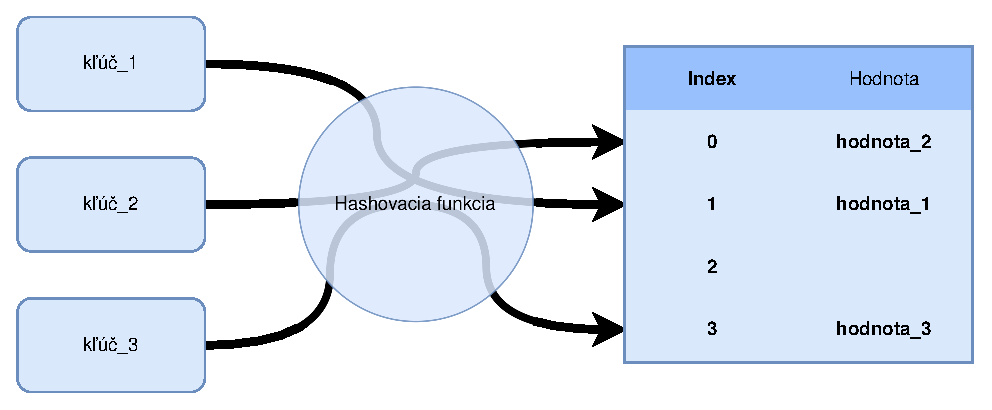
\includegraphics{img/hf}}
        \caption{Princíp hashovacej tabuľky}
        \label{fig:hf}
    \end{figure}
}

\section{Hashovacia funkcia}
\frame{
    \frametitle{Výber hashovacej funkcie}
    \begin{itemize}
        \item Využitím hashovania získavame rýchlosť vyhľadávania na úkor využívaného dátového priestoru.
        \item Najbežnejšie metódy hashovania: \textit{(podľa zložitosti)}
        \begin{enumerate}
            \item bitové operácie,
            \item násobenie,
            \item delenie.
        \end{enumerate}
        \item Okrem komplexnosti sa zohľadňuje najmä \textit{rovnomerná distribúcia odlišných kľúčov} medzi indexy.
        \item Príkladmi efektívnych hashovacích funkcií sú \textit{MurmurHash}\footnote{\href{https://en.wikipedia.org/wiki/MurmurHash}{https://en.wikipedia.org/wiki/MurmurHash}} alebo \textit{Fowler–Noll–Vo}\footnote{\href{https://w.wiki/XKZ}{https://w.wiki/XKZ}}
    \end{itemize}
}

\section{Synonymá}
\frame{
    \frametitle{Riešenie synoným}
    \textit{Čo s~rôznymi kľúčmi, ktoré sa namapujú na rovnaký index (\textbf{synonymá})?}
    \begin{itemize}
        \item \textbf{Explicitné} zreťazenie\,--\,napr. linerárny zoznam na každom indexe
        \item \textbf{Implicitné} zreťazenie\,--\,cieľový index získaný z~pôvodného indexu
    \end{itemize}
    \begin{figure}
        \centering
        \begin{subfigure}{0.5\textwidth}
          \centering
          \scalebox{0.5}{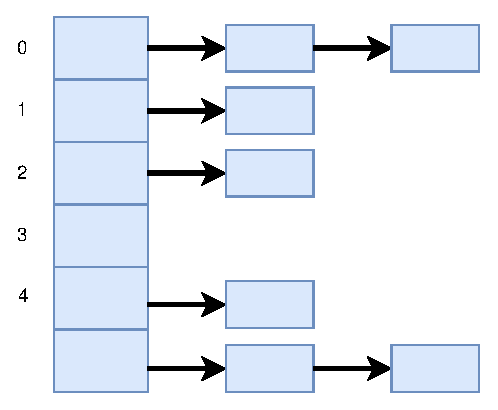
\includegraphics{img/expl}}
          \caption{Explicitné zreťazenie s~lineárnym zoznamom}
        \end{subfigure}%
        \begin{subfigure}{.5\textwidth}
          \centering
          \scalebox{0.5}{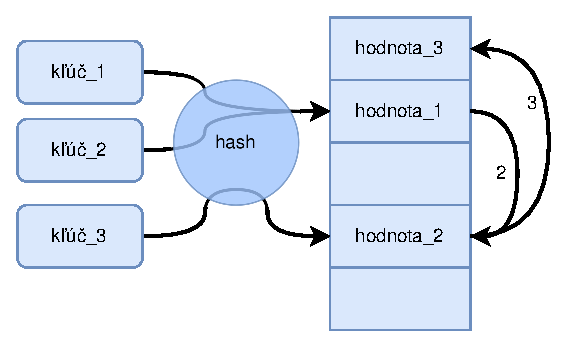
\includegraphics{img/impl}}
          \caption{Implicitné zreťazenie s~pevným\quad krokom~2}
        \end{subfigure}
    \end{figure}
}

\section{Operácie}
    \subsection{Search}
    \frame{
    \frametitle{Search}
        \textbf{Princíp:} Na príslušnom indexe prejdi zoznam prvkov a~vráť ten s~hľadaným kľúčom
        \begin{algorithm}[H]
            index = hashFunc(\texttt{KEY})\;
            bucket = hashTable[index]\;
            item = bucket.start\;
            \While{(item is not bucket.end)}{
                \uIf{(item.key is \texttt{KEY})}{
                    \Return item\;
                }
                \Else{
                    item = item.next\;
                }
             }
             \Return NOT\_FOUND;
         \caption{Vyhľadávanie prvku podľa kľúča \texttt{KEY}}
        \end{algorithm}
    }
    
    \subsection{Insert}
    \frame{
        \frametitle{Insert}
        \textbf{Princíp:} Na príslušnom indexe nájdi voľnú pozíciu a~vlôž na ňu nový prvok
        \begin{algorithm}[H]
            index = hashFunc(new\_item.\texttt{KEY})\;
            bucket = hashTable[index]\;
            item = bucket.start\;
            \While{(item is not bucket.end)}{
                \uIf{item is empty}{
                    item = new\_item\;
                    \textbf{return}\;
                }
                \Else{
                    item = item.next\;
                }
             }
         \caption{Vkladanie prvku s kľúčom \texttt{KEY}}
        \end{algorithm}
    }
    
    \subsection{Delete}
    \frame{
        \frametitle{Delete}
        \textbf{Princíp:} Na príslušnom indexe nájdi hľadaný prvok a~odstráň ho zo zoznamu
        \begin{algorithm}[H]
            index = hashFunc(new\_item.\texttt{KEY})\;
            bucket = hashTable[index]\;
            item = bucket.start\;
            \While{(item is not bucket.end)}{
                \uIf{(item.key is \texttt{KEY})}{
                    delete item\;
                    link item.previous and item.next\;
                    \textbf{return}\;
                }
                \Else{
                    item = item.next\;
                }
             }
             \Return NOT\_FOUND;
         \caption{Vymazanie prvku s kľúčom \texttt{KEY}}
        \end{algorithm}
    }

\frame{
    \section{Zdroje}
    \frametitle{Použité zdroje}
        \begin{thebibliography}{10}
            \bibitem[IAL]{ial}Predmet IAL\,--\,6. prednáška "Vyhledávací tabulky", FIT VUT, 2020
            
            \bibitem[Software Engineering at StackExchange]{hashfunc}Which hashing algorithm is best for uniqueness and speed?
            \newblock\url{https://softwareengineering.stackexchange.com/questions/49550/which-hashing-algorithm-is-best-for-uniqueness-and-speed}
        \end{thebibliography}
}


\end{document}
